%!TEX root = ../report.tex

\begin{document}
    \chapter{Results}
    In this chapter, we will discuss about the experiments conducted for out-of-distribution (OOD) detection on RandLA-Net using uncertainty techniques such as deep ensembles and flipout.
    These experiments were conducted on Semantic3D dataset as training in-distribution (ID) dataset and two datasets particularly S3DIS and Toronto3D are used as OOD datasets. 
    The detailed description about datasets can be found in Chapter \textcolor{red}{cite here}, about RandLA-Net in Section \textcolor{red}{cite here}, and about deep ensembles and flipout in Section \textcolor{red}{cite here}
    The list of experiments conducted to acheive OOD detection are as follows:
    \begin{enumerate}
        \item Train and evaluate the deep ensembles of RandLA-Net on Semantic3D dataset and discussed in Section \ref{sec:deepensemble_train}.
    \end{enumerate}

    %%%%%% Deep ensmebles performance gains experiment %%%%%%
    \section{Deep ensembles}
    \label{sec:deepensemble_train}
    \textbf{Aim:} Train multiple models of RandLA-Net with random initializations on Semantic3D dataset and combine the results from the get combined prediction. 
    These models are evlauated using mean Intersection-over-Union (mIOU) and Accuracy.

    \begin{table}[h!]
        \resizebox{\textwidth}{!}{%
        \begin{tabular}{c|c|cccccccc|c}
        %\textbf{\#Ensembles} & \textbf{MeanIOU} & \textbf{Accuracy} & \textbf{Manmadeterrain} & \textbf{Naturalterrain} & \textbf{Highvegetation} & \textbf{Lowvegetation} & \textbf{Buildings} & \textbf{Hardscapes} & \textbf{Scanningartifacts} & \textbf{Cars} \\ \hline
        & & \multicolumn{7}{c}{\textbf{IoU per class}} & \\ \hline
        \textbf{\#Ensembles} & \textbf{MeanIOU} & \textbf{C1} & \textbf{C2} & \textbf{C3} & \textbf{C4} & \textbf{C5} & \textbf{C6} & \textbf{C7} & \textbf{C8} & \textbf{Accuracy} \\ \hline
        1& 68.19& 94.55& 81.19& 84.67& 29.43& 81.37& 18.85& 64.74& 90.74& 88.78 \\
        5& 69.51& 94.73& 81.92& 84.42& 28.05& \textbf{86.41}& 28.50& 61.03& 91.03& 90.04 \\
        10& 69.97& 95.25& 83.73& 86.63& 30.36& 84.13& 18.60& \textbf{66.01}& 92.61& 89.94 \\
        15& 70.32& 95.27& 83.54& \textbf{88.22}& \textbf{32.19}& 84.82& 26.17& 61.67& 90.75& \textbf{90.57} \\
        20& \textbf{70.80}& \textbf{95.55}& \textbf{84.11}& 86.65& 29.60& 85.41& \textbf{29.58}& 62.47& \textbf{93.06}& 90.56 \\
        \end{tabular}%
        }
        \caption{Illustration of performance of RandLA-Net on Semantic3D over number of ensembles. meanIOU and IOU per class and overall accuracy are represented here.
        C1 to C8 are the classes of Semantic3D which are Manmadeterrain, Naturalterrain, Highvegetation, Lowvegetation, Buildings, Hardscapes, Scanningartifacts, and Cars.}
        \label{tab:ensemble_eval}
    \end{table}
    We trained 20 models of RandLA-Net over Semantic3D dataset with training procedure described in Section \textcolor{red}{cite here}.
    Table \ref{tab:ensemble_eval} represents the meanIoU, Accuracy and per class IoU with each row representing the performance value with ensemble size being multiple of 5.
    Figure \ref{fig:meaniou_de} and \ref{fig:acc_de} representing the performance with mIoU and Accuracy with all ensmebles respectively.
    Some of the predicted points clouds in comparison with ground truth are represented in Figure \textcolor{red}{cite here}.
    \begin{figure}[htbp]
        \begin{subfigure}{0.495\textwidth}
            \includestandalone[scale=0.95]{images/miou}
            \caption{}
            \label{fig:meaniou_de}   
        \end{subfigure}
        \begin{subfigure}{0.495\textwidth}
            \includestandalone[scale=0.95]{images/acc_de}
            \caption{}
            \label{fig:acc_de}
        \end{subfigure}
        \caption{Evaluation results of the deep ensemble of RandLA-Het on Semantic3D dataset with (a) representing the meanIoU over ensemble size and (b) representing accuracy over ensemble size.}
    \end{figure}

 

    %%%%%% Segmentation output here %%%%%%
    $$
    \text{\centering \Large\textbf{\textcolor{red}{Place the segmentation output here}}}
    $$
    %%%%%% Segmentation output here %%%%%%
    
    \textbf{Conclusions:}
    From this experiment, we draw the following conclusions 
    \begin{itemize}
        \item Deep ensembles improved the overall performance of the model significantly in terms of mIoU and Accuracy.
        \item Figure \ref{fig:sem3ddist} depicts low training points size for classes low vegetation, hardscapes, scanning artifacts and cars. Because of this classes low vegetation and hardscapes show less mIoU but use of deep ensembles improved their performance significantly.
        \item Eventhough cars are underrepresented in number of training points, efficient feature extraction of RandLA-Net helps in better segmentation of cars. As this is the same case in SemanticKITTI evaluation proposed in \cite{Hu_2020_CVPR_Randla}.
        \item From Figure \ref{fig:meaniou_de}, the performance gains in terms of mIOU after the ensemble size of 10 is minimal.
    \end{itemize}

    %%%%%% Maximum probability (Semantic3D vs S3DIS) %%%%%%
    \section{Probability-Semantic3D vs S3DIS}
    \label{sec:prob_sem3dvs3dis}
    \textbf{Aim: } In this experiment, we study how the probability scores are distributed in Semantic3D and S3DIS datasets which are ID and OOD datasets respectively.
    \begin{figure}[htbp]
        \begin{subfigure}{0.54\textwidth}
            \includestandalone[scale=0.9]{images/mean_prob_sem3dvs3dis}
            \caption{}
            \label{fig:prob_sem3dvs3dis}    
        \end{subfigure}
        \begin{subfigure}{0.45\textwidth}
            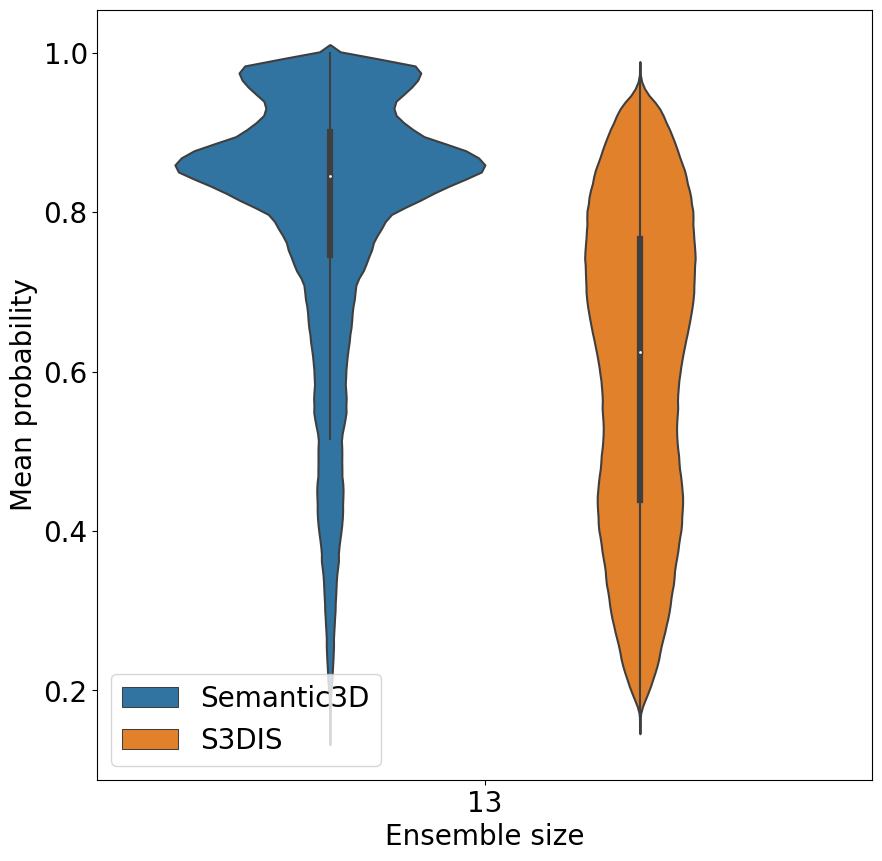
\includegraphics[scale=0.33]{images/violin_in_Max_predicted_probability.png}
            \caption{}
            \label{fig:13_sem3dvs3dis}
        \end{subfigure}
    \end{figure}

\end{document}
